% Tags: 4321102, flip, workings, table, flip-flop, flop
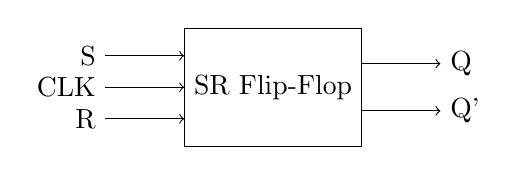
\begin{tikzpicture}[block/.style={rectangle, draw, minimum width=2cm, minimum height=1.5cm}]
    \node[block] (SRFF) at (0,0) {SR Flip-Flop};
    \draw[<-] (SRFF.west) ++(0,0.4) -- ++(-1,0) node[left] {S};
    \draw[<-] (SRFF.west) ++(0,0) -- ++(-1,0) node[left] {CLK};
    \draw[<-] (SRFF.west) ++(0,-0.4) -- ++(-1,0) node[left] {R};
    \draw[->] (SRFF.east) ++(0,0.3) -- ++(1,0) node[right] {Q};
    \draw[->] (SRFF.east) ++(0,-0.3) -- ++(1,0) node[right] {Q'};
\end{tikzpicture}
